
\subparagraph{Potenziale vettore di una spira a grande distanza}
Si ricorda l'espressione del vettore potenziale
$$
\vec{A}(p) = \frac{\mu_0}{4\pi}\hat{m}\times\frac{\vec{e}_r}{r_p^2} = \frac{\mu_0}{4\pi}\vec{m}\times\frac{\vec{r}_p}{r_p^3} = -\frac{\mu_0}{4\pi}\vec{m}\times\nabla_p \left(\frac{1}{r_p} \right)
$$
È quindi possibile calcolare il campo $\vec{B}$ effettuando il rotore di $\vec{A}$
$$
\vec{B}(p) = \nabla\times\vec{A} = -\frac{\mu_0}{4\pi}\nabla_p\times\left(\vec{m}\times\nabla_p\left(\frac{1}{r_p}\right)\right)
$$
Identità vettoriale: $\nabla\times(f\vec{v}) = f\nabla\times\vec{v} + \nabla f \times \vec{v}$
$$
f = \frac{1}{r_p} \qquad \vec{v}=\vec{m}
$$
quindi
$$
\nabla\times\left(\frac{\vec{m}}{r_p}\right) = \frac{1}{r_p}\nabla\times\vec{m} + \nabla\left(\frac{1}{r_p}\right)\times \vec{m} = \frac{1}{r_p}\nabla\times\vec{m} - \vec{m}\times\nabla\left(\frac{1}{r_p}\right)
$$
L'ultimo termine può essere sostituito nell'espressione del campo ma il rotore rispetto
a $p$ del rotore di $\vec{m}$ è nullo quindi
$$
\vec{B}(p) = \frac{\mu_0}{4\pi} \nabla_p\times\nabla_p\times\left(\frac{\vec{m}}{r_p}\right)
$$
ma il rotore del rotore è il gradiente della divergenza meno il laplaciano vettore
$$
\vec{B}(p) = \frac{\mu_0}{4\pi} \left[\nabla\left(\nabla\cdot\left(\frac{\vec{m}}{r_p}\right)\right) - \cancel{\nabla^2\left(\frac{\vec{m}}{r_p}\right)}\right]
$$
Il laplaciano di $\frac{\vec{m}}{r_p}$ è nullo in quanto il momento magnetico $\vec{m}$ è 
costante come il potenziale di una carica puntiforme
$$
\vec{B}(p) = \frac{\mu_0}{4\pi}\nabla\left(\nabla\cdot\left(\frac{\vec{m}}{r_p}\right)\right) = \frac{\mu_0}{4\pi}\nabla\left(\vec{m}\cdot\nabla\left(\frac{1}{r_p}\right)\right)
$$
l'espressione tra parentesi può essere nominata $\psi$, un caso in cui il campo magnetico
può essere espresso mediante un potenziale magnetico scalare, dato che $\psi$ è una funzione 
scalare.
$$
\psi(p) = \frac{\mu_0}{4\pi}\vec{m}\cdot\nabla\left(\frac{1}{r_p}\right) = -\frac{\mu_0}{4\pi}\vec{m}\cdot \frac{\vec{r_p}}{r_p^3}
$$
Così come il potenziale di un dipolo elettrico era
$$
V(p) = \frac{1}{4\pi\varepsilon_0} \vec{p}\cdot\frac{\vec{r}_p}{r_p^3}
$$
Ciò significa che a meno di costanti e unità di misura, a grande distanza le linee di
campo magnetico prodotte da una spira circolare percorsa da corrente sono identiche alle
linee di campo elettrico prodotte da un dipolo.
\newpage
\subsection{Coefficienti di auto e mutua induzione per circuiti quasi-filiformi}
Siano presenti una serie di spire attraversate da corrente, si associano delle superfici
di orlo ad ogni linea orientate.
\begin{figure}[H]
\centering
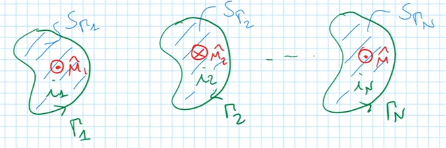
\includegraphics[width = 0.4\linewidth]{circuiti_auto_mutua_induzione}
\end{figure}
Per calcolare il campo si usa il PSE, il flusso attraverso la superficie $k$ si calcola
con 
$$
\Phi_k = \iint_{S_{\Gamma_k}}\vec{B}\cdot\hat{n}_k dS
$$
Il campo totale si può trovare con il potenziale vettore generato dalle spire
$$
\vec{A}(p) = \frac{\mu_0}{4\pi}\oint_{\Gamma_1} \frac{i_1\hat{t}_1(p')}{|\vec{r}_p - \vec{r}_{p'}|}dl_1 + ... + \frac{\mu_0}{4\pi}\oint_{\Gamma_N} \frac{i_N\hat{t}_n(p')}{|\vec{r}_p-\vec{r}_{p'}|}dl_N
$$
Sostituendo
$$
\Phi_k = \iint_{S_{\Gamma_k}} \nabla\times\vec{A}\cdot\hat{n}dS \stackrel{\text{T. di Stokes}}{=} \oint_{\Gamma_k}\vec{A}\cdot\hat{t}_kdl_k
$$
$$
\Phi_k = \oint_{\Gamma_k} \left[\frac{\mu_0}{4\pi} \oint_{\Gamma_1} \frac{i_1\hat{t}_1(p')}{|\vec{r}_p - \vec{r}_{p'}|}dl_1 + ... + \frac{\mu_0}{4\pi}\oint_{\Gamma_N} \frac{i_N\hat{t}_N(p')}{|\vec{r}_p - \vec{r}_{p'}|}dl_N \right]\cdot \hat{t}_k(p) dl_k
$$
Ma $t_k(p)$ non dipende da $p'$ si può portare all'interno degli integrali mentre
le correnti sono costanti e possono invece essere portate fuori
$$
\Phi_k = \sum_{j=i}^N \left(\frac{\mu_0}{4\pi} \oint_{\Gamma_k}\oint_{\Gamma_j} \frac{\hat{t}_j(p')\cdot\hat{t}_k(p)}{|\vec{r}_p-\vec{r}_{p'}|} dl_j dl_k \right)i_j
$$
Il termine tra parentesi è tutto sommato uno scalare che dipende da due indici quindi lo 
riassumiamo con $L_{kj}$
$$
\Phi_k = \sum_{j=i}^N L_{kj} i_j
$$
Il coefficiente prende nomi differenti
$$
\begin{cases}
L_{kk} & \text{Coefficiente di autoinduzione della spira } k\\
L_{kj} & \text{Coefficiente di mutua induzione tra la spira } k \text{ e } j
\end{cases}
$$
Combinando tutti i coefficienti si ottiene una matrice $N\times N$ di coefficienti definiti
$$
L_{kj} = \left.\frac{\Phi_k}{i_j}\right|_{i_S = 0,\ S\neq j}
$$
Il flusso che l'avvolgimento $j$ produrrebbe da solo concatenato con $k$ se la corrente
$i_j$ agisse da sola con tutte le altre uguali a zero ossia l'effetto nel circuito $k$
della causa nel circuito $j$.

Una proprietà analoga si ritrova nei doppi bipoli resistivi che godono della proprietà di
reciprocità per il \href{https://it.wikipedia.org/wiki/Teorema_di_Tellegen}{teorema di Tellegen} ossia che il rapporto tra causa ed effetto tra due circuiti diversi è uguale.

Si vede dunque che $L_{kj} = L_{jk}$ perché negli integrali è presente il prodotto
scalare tra i versori $\hat{t}_j$ e $\hat{t}_k$ che gode della proprietà commutativa,
inoltre si invertirebbero tutti gli indici degli integrali.

Il coefficiente di autoinduzione $L_{kk}$ è intrinsecamente positivo dato che 
l'orientamento del campo 
è concorde con l'orientamento della curva se quest'ultimo rispetta il verso della corrente.
Ciò non è sempre vero se gli avvolgimenti sono diversi dato gli orientamenti delle 
linee sono indipendenti tra loro.

\textbf{Osservazione:} il circuito non può essere realmente filiforme perché avrebbe al suo
interno un campo che divergerebbe sulla linea e $L_{kk}$ andrebbe a infinito.

\subsection{Bilancio energetico di una spira percorsa da correnti stazionarie}
Si suppone che ci sia un generatore collegato ad una spira nella quale circola una corrente
$i$ e di linea media $\Gamma$.
\begin{figure}[H]
\centering
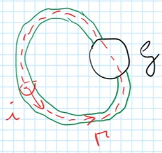
\includegraphics[width = 0.3\linewidth]{faraday_neumann_spira}
\end{figure}
Si suppone che la corrente vari \textit{lentamente} (caso quasi-stazionario), applicando Faraday-Neumann
$$
\oint_\Gamma \vec{E}\cdot\hat{t}dl = -\frac{d}{dt}\iint_{S_\Gamma}\vec{B}\cdot\hat{n}dS = 
-\frac{d}{dt}\Phi_\Gamma
$$
la corrente è sostenuta dal generatore quindi
$$
\vec{J} = \gamma(\vec{E}+\vec{E}_m) \Rightarrow \vec{E} = \eta \vec{J} - \vec{E}_m
$$
Sostituendo si ottiene
\begin{equation}
\oint_\Gamma \eta\vec{J}\cdot\hat{t}dl - \oint_\Gamma \vec{E}_m\cdot\hat{t}dl = - \frac{d}{dt} \Phi_\Gamma
\label{eq:faraday-neumann}
\end{equation}
ma $\Phi_\Gamma = Li$ 
$$
L = \frac{\mu_0}{4\pi}\oint_\Gamma\oint_\Gamma \frac{\hat{t}(p')\cdot\hat{t}(p)}{|\vec{r}_p-\vec{r}_{p'}|} dldl'
$$
La (\ref{eq:faraday-neumann}) diventa
$$
Ri + R_i i - e_0 = -L\frac{di}{dt} \Rightarrow e_0 = (R+R_i) + L\frac{di}{dt}
$$
Ossia la classica equazione R-L con un generatore di tensione reale.
Se si moltiplicano entrambi i membri per $i dt$
$$
e_0idt = (R+R_i) i^2 dt + \frac{d}{dt} \left(\frac{1}{2}Li^2\right)dt
$$
integrando membro a membro tra due istanti di tempo $(0,t)$
\begin{equation}
\int_0^t e_0 i dt = \int_0^t (R+R_i) i^2 dt + \frac{1}{2}Li^2(t) - \frac{1}{2} L i^2 (0)
\label{eq:bilancio_energia}
\end{equation}
$$
\Delta W^{(e)}_{\text{gen}} (0,t) = \Delta W^{(a)}_{R+R_i} (0,t) + \Delta W^{(a)}_L(0,t)
$$
Definita la funzione $w_m(t) = \frac{1}{2}Li^2(t)$ ha il significato di energia 
immagazzinata nel campo magnetico della spira all'istante $t$.

Se si suppone che $i(t=0) = 0$ allora l'ultimo termine nella (\ref{eq:bilancio_energia}) è 
nullo e si vede che l'energia fornita dal generatore viene in parte dissipata dai resistori
interno e della spira e in parte immagazzinata dall'induttore.

Si esprime ora l'energia immagazzinata in termini di campi
$$
w_m(t) = \frac{1}{2}Li^2 = \frac{\mu_0}{4\pi}\frac{1}{2}\oint_\Gamma\oint_\Gamma \frac{\hat{t}(p')\cdot\hat{t}(p)}{|\vec{r}_p-\vec{r}_{p'}|}dl'dl\ i^2
$$
ma
$$
\frac{i}{S}\hat{t}dl = \vec{J}dV
$$
quindi
$$
w_m(t) = \frac{\mu_0}{4\pi}\frac{1}{2}\oint_\Gamma\oint_\Gamma \frac{\vec{J}(p')dV}{|\vec{r}_p-\vec{r}_{p'}|}\cdot \vec{J}(p)dV
$$
(manca un $S^2$?)

Si vede che 
$$
\oint_\Gamma \frac{\vec{J}(p')dV}{|\vec{r}_p-\vec{r}_{p'}|} = \frac{4\pi}{\mu_0}\vec{A}(p)
$$
quindi
$$
w_m(t) = \frac{1}{2}\iiint_\Omega \vec{J}(p)\cdot\vec{A}(p)dV
$$
dove $\Omega$ è la regione occupata dalla spira. Ricordando che $\vec{J} \neq 0$ solo in 
$\Omega$ si può estendere l'integrale in tutto lo spazio.
$$
w_m(t) = \frac{1}{2}\iiint_{\Omega_\infty} \vec{J}\cdot\vec{A}dV
$$
Dalle equazioni di Maxwell $\nabla\times\vec{B} = \mu_0\vec{J} \Rightarrow \vec{J} = \frac{\nabla\times\vec{B}}{\mu_0}$
$$
w_m(t) = \frac{1}{2}\iiint_{\Omega_\infty} \frac{\nabla\times\vec{B}}{\mu_0}\cdot\vec{A}dV
$$
Si ricorda l'identità $\nabla\cdot(\vec{A}\times\vec{B}) = \vec{B}\cdot\nabla\times\vec{A}
- \vec{A}\cdot\nabla\times\vec{B}$

Quindi $\vec{A}\cdot(\nabla\times\vec{B}) = \vec{B}\cdot\nabla\times\vec{A} - \nabla\cdot(\vec{A}\times\vec{B})$ si sostituisce nell'integrale
$$
w_m(t) = \frac{1}{2}\iiint_{\Omega_\infty}\frac{\vec{B}}{\mu_0}\cdot\nabla\times\vec{A} dV - \cancel{\frac{1}{2}\iiint_{\Omega_\infty}\frac{1}{\mu_0} \nabla\cdot(\vec{A}\times\vec{B})dV}
$$
Il secondo termine è l'integrale della divergenza di un vettore, applicando il teorema
della divergenza questo equivale a
$$
\frac{1}{2\mu_0}\iiint_{\Omega_\infty} \nabla\cdot(\vec{A}\times\vec{B})dV = \frac{1}{2\mu_0}\iint_{\partial\Omega_\infty} \vec{A}\times\vec{B}\cdot\hat{n}dS \to 0 \text{ all'infinito}
$$
ma il potenziale $\vec{A}$ e il campo $\vec{B}$ sono normali all'infinito. 
In conclusione
$$
w_m(t) = \frac{1}{2}\iiint_{\Omega_\infty} \frac{B^2}{\mu_0}dV
$$
La funzione $\frac{1}{2}\frac{B^2}{\mu_0} $ è la densità di energia magnetica 
immagazzinata.
\newpage
\subsection{Due circuiti accoppiati}
Siano presi due circuiti percorsi da corrente
\begin{figure}[H]
\centering
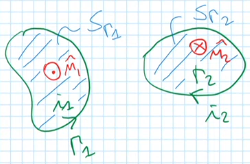
\includegraphics[width = 0.3\linewidth]{induzione_due_circuiti}
\end{figure}
Si hanno le seguenti relazioni
\begin{align*}
\Phi_1 & = L_1i_1 + M_{12}i_2 \\
\Phi_2 & = M_{21}i_1 + L_2i_2
\end{align*}
ma $M_{12} = M_{21} = M$ e supponendo che entrambe le spire contengano un generatore, 
svolgendo il bilancio energetico e sommando le equazioni si ottiene
\begin{align*}
e_{01}i_1dt &  = \left(R_1+R_{i1}\right)i_1^2dt + \frac{d}{dt} \left(L_1 i_1 + Mi_2 \right)i_1 dt \\
e_{02}i_2dt &  = \left(R_2+R_{i2}\right)i_2^2dt + \frac{d}{dt} \left(M i_1 + L_2i_2 \right)i_2 dt 
\end{align*}
$$
(e_{01}i_1 + e_{02}i_2) dt = \left[(R_1+R_{i1})i_1^2 + (R_2+R_{i2})i_2^2 \right]dt + 
\frac{d}{dt}\left[ \frac{1}{2}L_1i_1^2 + \frac{1}{2}L_2i_2^2 + Mi_1i_2 \right]
$$
L'ultimo termine è proprio $w_m(t)$ l'energia magnetica immagazzinata nel campo di 
induzione magnetica $\vec{B}$ prodotto dai due circuiti.
$$
w_m(t) =  \frac{1}{2}L_1i_1^2 + \frac{1}{2}L_2i_2^2 + Mi_1i_2 =\frac{1}{2}\iiint_{\Omega_\infty} \frac{B^2}{\mu_0}dV \geq 0
$$
Non conta il verso delle correnti, se l'integrale è maggiore o uguale di zero a causa
della positività dell'integrando, allora anche il termine circuitale equivalente sarà
maggiore o uguale a zero.

Esiste dunque una condizione di fisica realizzabilità di due avvolgimenti (di un 
trasformatore) che afferma
$$
M^2 \leq L_1L_2
$$
Quando $M^2 = L_1L_2$ si parla di \textit{accoppiamento perfetto} altrimenti 
\textit{accoppiamento non perfetto}
\newpage
\subparagraph{Nel caso di N circuiti accoppiati}
$$
w_m(t) = \frac{1}{2}\sum_{k=1}^N \sum_{j=1}^N i_k L_{kj} i_j
$$
È la forma quadratica associata alla matrice dei coefficienti di auto e mutua induzione
$$\frac{1}{2}\cdot
\begin{bmatrix}
i_1 & \cdots & i_N
\end{bmatrix} \cdot
\begin{bmatrix}
L_{11} & \cdots & L_{1N} \\
\vdots & \ddots & \vdots\\
L_{N1} & \cdots & L_{NN}
\end{bmatrix} \cdot
\begin{bmatrix}
i_1 \\
\vdots \\
i_N
\end{bmatrix} = \frac{1}{2} \underline{i}^T\cdot\underline{\underline{L}}\cdot\underline{i}
$$

\subsection{Induttanza per unità di lunghezza di un cavo coassiale}
Può essere immaginato come due cilindri conduttori di raggio differente che giacciono
sullo stesso asse ad esempio $x$. La corrente circola nel conduttore interno in un verso
e sul conduttore esterno in verso opposto.

Per valutare il flusso e quindi l'induttanza per unità di lunghezza è necessario immaginare
una linea che connetta entrambi i conduttori orientata come in figura.
\begin{figure}[H]
\centering
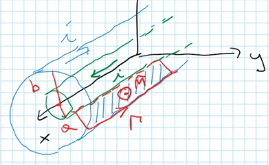
\includegraphics[width = 0.4\linewidth]{induttanza_cavo_coassiale}
\end{figure}
La superficie racchiusa dalla linea $\Gamma$ è anch'essa orientata secondo la regola della 
mano destra.

Per calcolare il flusso è necessario conoscere il campo $\vec{B}$ che sarà orientato in modo concorde alla superficie $S_\Gamma$
$$
\vec{B} = \frac{\mu_0 i }{2\pi r}\hat{n}
$$

Il flusso sarà quindi
$$
\Phi_\Gamma = \iint_{S_\Gamma} \vec{B}\cdot\hat{n}dS = \int_0^l dx\int_a^b \frac{\mu_0 i}{2 \pi r} dr = l \frac{\mu_0}{2\pi} i \ln\left(\frac{b}{a}\right)
$$
Il coefficiente di autoinduzione per unità di lunghezza sarà
$$
\frac{L}{l} = \frac{\Phi_\Gamma}{l\ i } = \frac{\mu_0}{2\pi} \ln\left(\frac{b}{a}\right)
$$
Si vede l'analogia con la capacità del condensatore cilindrico per unità di lunghezza
$$
\frac{C}{l} = \frac{2\pi\varepsilon_0}{\ln\left(\frac{b}{a}\right)}
$$
Eseguendo il prodotto di questi due termini
$$
\frac{L}{l}\frac{C}{l} = \frac{\mu_0}{\cancel{2\pi}}\cancel{2\pi}\varepsilon_0 = \mu_0 
\varepsilon_0 = \frac{1}{c^2}
$$
ma $c$ è una costante ed è proprio la velocità della luce nel vuoto \SI{3e8}{\meter/\second}.

Questo risultato fa  capire che se non si trascurano gli effetti propagativi, la 
propagazione dei campi elettromagnetici avviene alla velocità della luce nel vuoto.
